\chapter{Methodology}
% information on the corpus and writing data
%define  features that I will use for classification how I decided on this and motivation behind these features.
%%%%%%%%%%%%%%%%%%%%%%%%%%%%%%%%%%%%%%%%
\section{Characteristics of Japanese}
%%%%%%%%%%%%%%%%%%%%%%%%%%%%%%%%%%%%%%%%

The agglutinative nature of Japanese coupled with the absence of explicit word delimiters, presents challenges for
accurate word segmentation. Furthermore, the use of three distinct writing systems
\footnote{Hiragana, Katakana, and Kanji} leads to considerable orthographic variation. for instance, learners at
lower proficiency levels frequently rely on the phonetic alphabets (hiragana and katakana), which can exacerbate
segmentation and tokenization errors. This phenomenon has been observed in previous studies
\citep{yang1998, nagata2009}, where systems demonstrated a lack of robustness against "spelling" errors or the
erroneous use of kanji.

Defining a "word" in Japanese also differs considerably from Indo-European languages. While a bound morpheme in
Enlgish might be treated as a indificual word. this is generally not the case in Japanese. For example,
segmentation can be difficult.
With 3
alphabets used there can orthographic variation is also fairly common. Learners at the lower proficentcy levels
mostly will write using the phonetic alphabets hiragana and katakana sometimes leading to errors in
segmentation/tokenization as was observed in \citep{yang1998, nagata2009}.

What is considered a word in Japanese may differ from other languages european languages. While a bound morpheme in
English might be treated
as an individual word, this is generally not the case in Japanese. For example, the word 話す\textit{hanasu}(to speak)
is considered a single word. However its potential form, 話せる \textit{hanaseru}(to be able to speak) is often analyzed as
two distinct morphemes: 話\textit{hana} and せる\textit{seru}. Initial abalyses using the chose tokenizer and parser
revealed inconsistencies in this regard. Similar inconsistencies were observed with compound verbs, such as
言い切る(\textit{iikiru}, "to completely say\footnote{\textit{to say without restraint}}"). While this was consistently
split into 言い(\textit{ii}"to say") and 切る(\textit{kiru} a suffix indicating completion), other instances were
segmented into
食べ (\textit{tabe}"to eat") 切る(\textit{kiru}"completely"). These inconsistencies pose significant hurdles for the
reliable extraction of specific grammatical forms for criterial features and can lead to unreliable counts for
complexity measures.
% maybe say something about taking this into consideration when writing rules for criterial features.

%%%%%%%%%%%%%%%%%%%%%%%%%%%%%%%%%%%%%%%%
\section{About the International Corpus of Japanese as a Second Language(I-JAS)}
%%%%%%%%%%%%%%%%%%%%%%%%%%%%%%%%%%%%%%%%

This study utilizes data from the International Corpus of Japanese as a Second Language (I-JAS), as
detailed in
\citet{Sakoda2020}, was
used.  The
I-JAS corpus is comprised of both spoken and written samples of Japanese.  It includes data from a diverse pool of 1,
000 adult learners
(aged
between 17 and 63 years old), all of whom are learning Japanese as a second language. 50 Native speaker samples are also
included in the corpus as a control group.

Participant's proficiency levels were assessed using the Japanese Computer Adaptive Test (J-Cat)
\citep{Imai2009}, with Further details about this assessment is provided in the
subsequent
section \ref{j-cat}. In addition to proficiency scores, the corpus includes various metadata for each participant,
such as
their
native language,
prior experience of visiting or living in Japan, and current geographical location (whether outside or within Japan).

%%%%%%% This part below contains information only on the essay writing samples I previously analyzed. I have also
%%%%%%% included additional writing samples added to the corpus which has brought the total particiapnt pool to 1000
%%%%%%% again.
Writing samples were extracted from the larger I-JAS corpus. Samples  were provided from 687 individuals, including the
control group
of 50 native speakers. A detailed breakdown of the of the participants in the writing sample subset, categorized by
their corresponding Japanese Language Proficiency Test (JLPT) levels, is presented in \ref{tab:participants-chart}.

%Name: count, dtype: int64
\begin{table}[h!]
\centering
\begin{tabular}{cc}
\hline \textbf{JLPT Proficiency Level} & \textbf{\# of Participants} \\ \hline
N5 & 176 \\
N4  & 318 \\
N3 & 297\\
N2 & 165 \\
N1 & 44 \\
Native Speakers & 50 \\
\hline
\end{tabular}
\caption{\label{tab:participants-chart} Distribution of participants across JLPT proficiency levels. J-cat scores have been mapped to their equivallent JLPT levels. }
\end{table}

%%%%%%%%%%%%%%%%%%%%%%%%%%%%%%%%%%%%%%%%
\subsection{The Japanese Computerized Adaptive Test (J-CAT)}
\label{j-cat}
%%%%%%%%%%%%%%%%%%%%%%%%%%%%%%%%%%%%%%%%

%background and information on the J-CAT test compare to JLPT.

The Japanese Computerized Adaptive Test (J-CAT) \citep{Imai2009}, is a computer-administered assessment
designed to evaluate an
individual's proficiency in the Japanese language. While formerly freely accessible, the J-CAT is now overseen by
the  日本語教育支援協会(Japanese Language Education Support Association (JaLESA)). Japanese
universities frequently
employ the J-CAT as an efficient tool and flexible tool for placing foreign students into appropriate Japanese
language courses, primarily due to its on-demand administration compared to the JLPT which is only
administered bi-annually.

The adaptive nature of the J-CAT allows it to tailor question difficulty based on a student's performance across
four core areas: Vocabulary, Grammar, Listening, and Reading. Each participant receives a numberial score, which is
then mapped to one of seven distinct proficiency levels. These levels have been correlated with equivalent JLPT
scores, as detailed in \ref{tab:proficency-table}. For this study participants were categorized according to their
assigned JLPT level. Native speaker participants were assigned a default J-CAT score of 999.

\begin{figure}[h!]
    \centering
    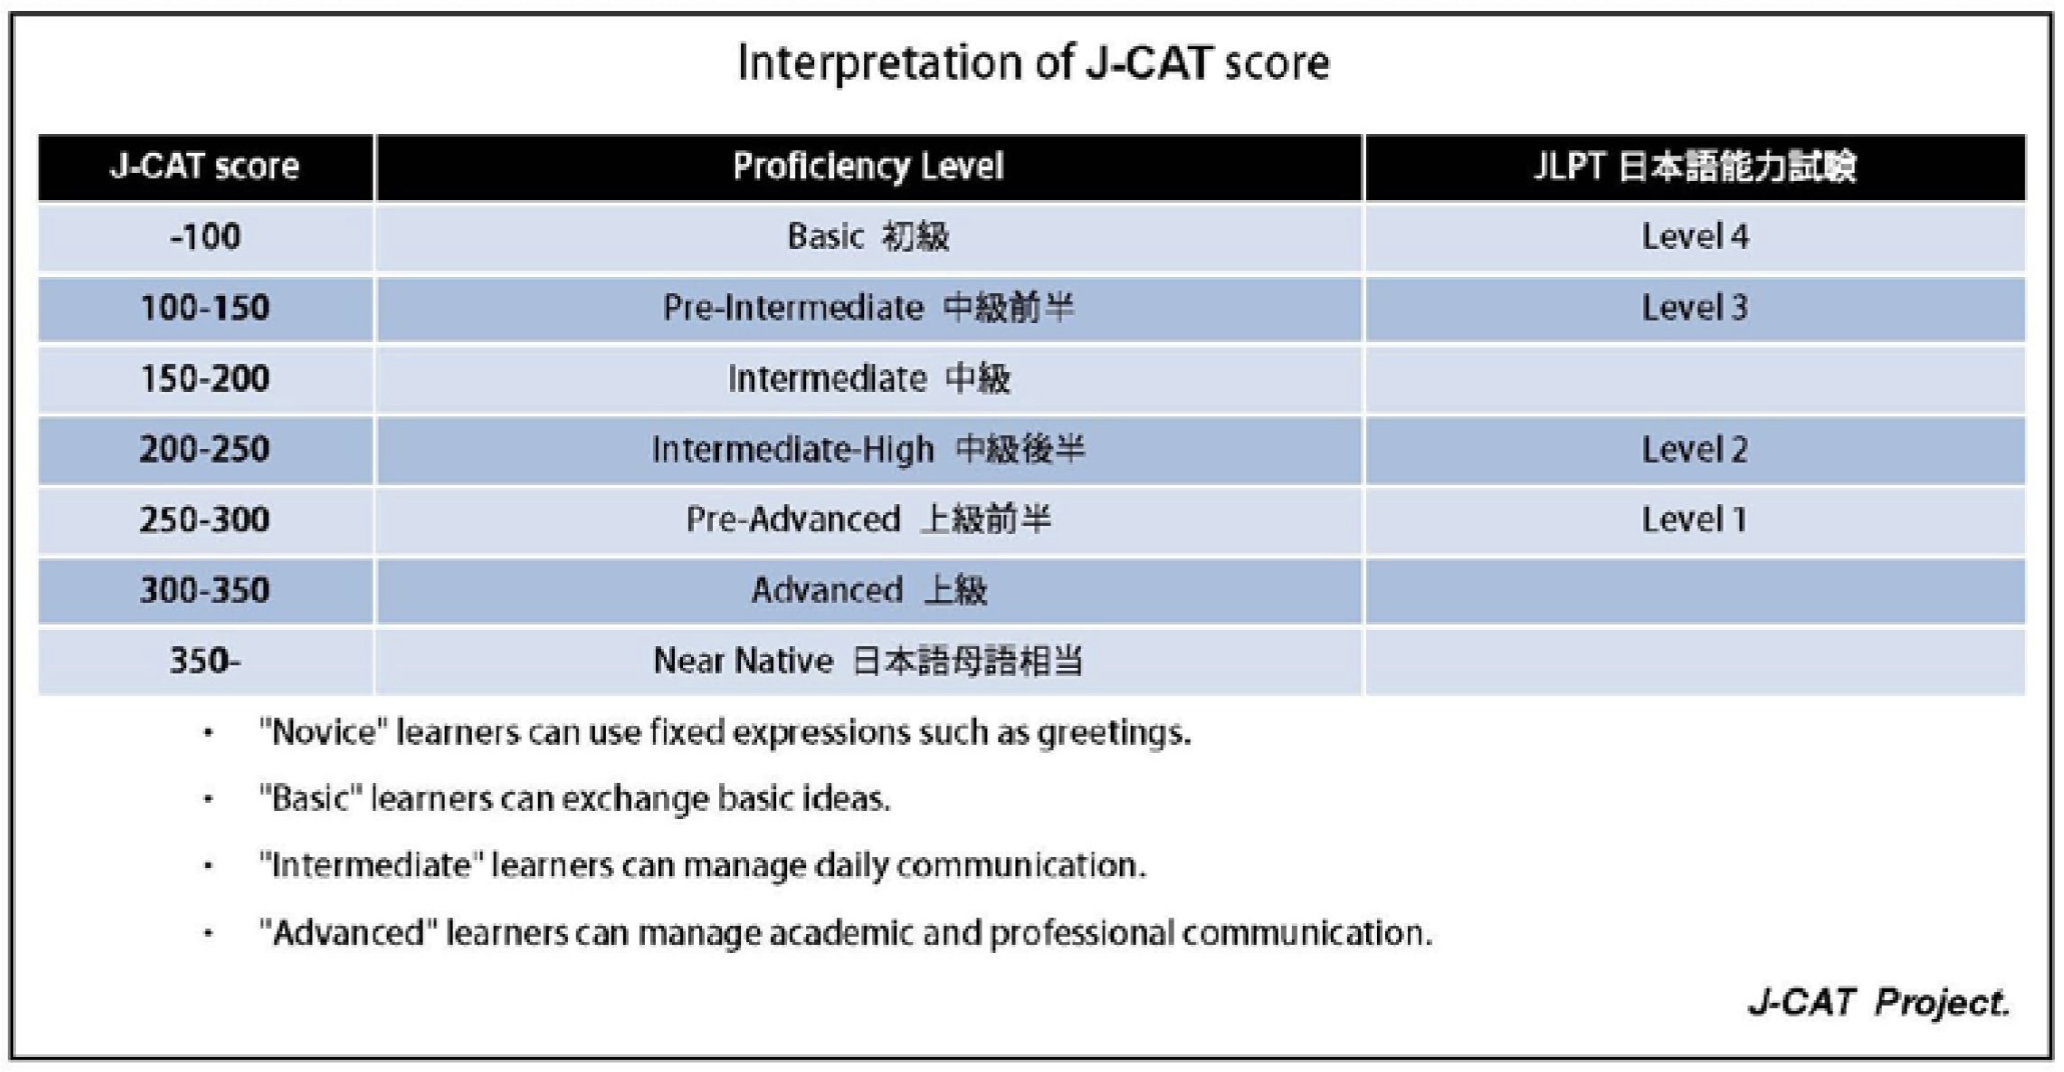
\includegraphics[scale=.3]{img/JCatScores.png}
    \caption[J-Cat Proficency Levels]{The assigned proficency levels from the J-Cat test as presented in the original paper in  2009. It is important to note that JLPT equivalencies do not align with the current JLPT framework, which was reformed in 2010. A revised score interpretation, connecting J-CAT scores to the updated JLPT levels, was released in 2011 and is provided in Table \ref{tab:proficency-table} }
    \label{fig:JCatLevels}
\end{figure}


\begin{table}[h!]
\centering
\begin{tabular}{lrl}
\hline \textbf{JLPT Proficiency Level} & \textbf{J-Cat Score}  \\ \hline
N5 & 0 - 149 \\
N4 & 150 - 199 \\
N3 & 200 - 249 \\
N2 & 250 - 299 \\
N1 & 300 - \\
Native & 999
\hline
\end{tabular}
\caption[Proficency Levels]{JLPT proficency level classification based on J-cat score ranges, adapted from
\cite{jcat_interpretation_guide}.}
\label{tab:proficency-table}
\end{table}

%%%%%%%%%%%%%%%%%%%%%%%%%%%%%%%%%%%%%%%%
\subsection{Writing Tasks}
%%%%%%%%%%%%%%%%%%%%%%%%%%%%%%%%%%%%%%%%

% add the additional SW 1 and 2 tasks where participants were expected to write a story based on a picture.
Each participant submitted up to six samples of writing for specific tasks, detailed below that were designed to
elicit a variety of linguistic responses across different discourse types and levels of formality:
\begin{itemize}
    \item A short essay titled "Our Eating Habits," requiring a comparatie analysis of fast food and home-cooked
    meals within the context of the learner's home country.
    \item A formal letter addressed to a former teacher, requesting a letter of recommendation for a scholarship
    application.
    \item An email seeking an extension for a report submission deadline.
    \item An apology email declining an invitation
    \item A story-telling task (Story Writing 1), where the learner was expected to narrate a story based on a
    series of pictures depicting a picnic theme. Sample images for this task are also shown in Figure \ref{fig:ST}.
    \item A story telling task (Story Writing 2) where the learner was expected to narrate a story based on a
    series of pictures depicting a lost key. Sample images for this task can be seen in Figure \ref{fig:ST}.
\end{itemize}

These tasks were standardized across all participants, regardless of their proficiency levels, encompassing a range
of communicative functions and formalities. While the possiblity of a "task effect" as observed in
\citet{Alexpoulou2017} is possible due to certain tasks requiring the use of certain forms, as the tasks are
consistent across proficency levels,
this consistency allows for a direct observation of the linguistic forms learners use at different proficiency
levels. Consequently, all writing samples within the corpus were processed as-is, without any correction of learner
errors.

\begin{figure}[h!]
    \centering
    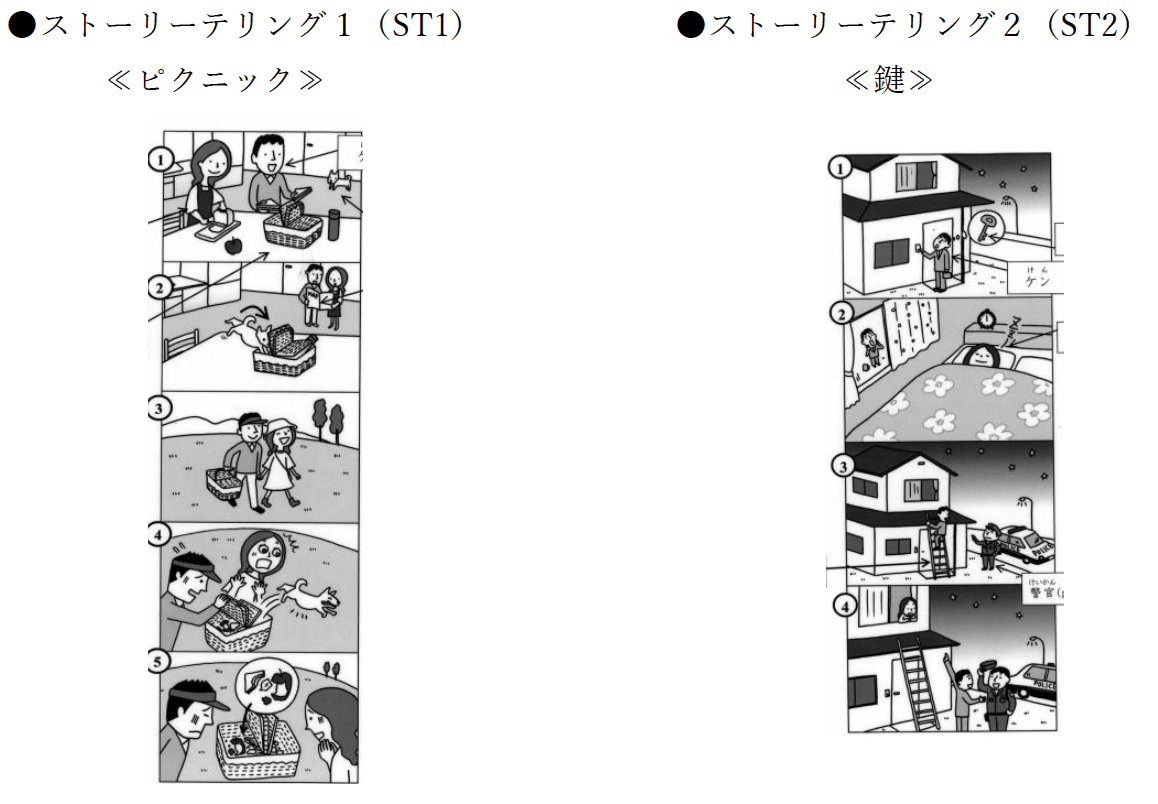
\includegraphics[scale=.45]{img/ST.png}
    \caption[Story Telling Tasks]{Images used for the two story-telling tasks. Learners were instructed to construct a narrative based on these visual prompts. }
    \label{fig:ST}
\end{figure}

%%%%%%%%%%%%%%%%%%%%%%%%%%%%%%%%%%%%%%%%
\subsection{Text Preprocessing}
%%%%%%%%%%%%%%%%%%%%%%%%%%%%%%%%%%%%%%%%

%Mention the preprocessing of the text. Talk about spacys' ginza pipeline used for parsing-tagging etc.
The raw text data from each writing sample underwent a comprehensive preprocessing pipeline. Given the specific
challenges of Japanese text processing, particularly for learner language where standard NLP tools may not be
robust, Spacy's Ginza package \cite{Ginza} (v 5.2) a Japanese language model for spaCy for Japanese was employed.
Ginza was selected for its comprehensive capabilities in handling Japanese text, including tokenization,
Part-of-Speech(POS) tagging, depedency parsing, lemmatization, morphological analysis, and its integration with
spaCy's rule based matcher.

For certain morphological lexical and measures, punctuation was removed from the text to prevent its influence on
token counts and other analyses. All characters in the writing were first converted to full-size characters \footnote{This is to prevent any errors due to unintentional half-size characters that may have been included in the writings when converting between different formating. For this the mojimoji package was used https://pypi.org/project/mojimoji/}, then
the texts were tokenized, tagged for parts-of-speech,
Lemmatizatized, dependency parsed.

The corpus for this study comprises over 4,840 uncorrected samples of writing from the participants, necessitating
the reliance on measures that can be automatically calculated.
 The algorithms for calculating various complexity measures and criterial features, discussed in subsequent
sections, were
were developed by the author based on the output of this preprocessing pipeline. The source code for these
algorithms in publicly available at: \href{https://github.com/meghorikawa/JFE}{https://github.com/meghorikawa/JFE} }.

%%%%%%%%%%%%%%%%%%%%%%%%%%%%%%%%%%%%%%%%
\section{Complexity Measures}
%%%%%%%%%%%%%%%%%%%%%%%%%%%%%%%%%%%%%%%%

Complexity measures were chosen for a multi-dimensional approach to cover multiple linguistic domains including
Lexical, Syntactic, Morphological. Below I will detail the measures chosen for each domain


%%%%%%%%%%%%%%%%%%%%%%%%%%%%%%%%%%%%%%%%
\subsection{Syntactic Complexity Measures}
%%%%%%%%%%%%%%%%%%%%%%%%%%%%%%%%%%%%%%%%
Sent Length, Clauses per sentence, Noun phrase length,  Subordination, coordination, noun phrase length, MDD, MHD

Describe any motivation for each - how I extracted them/calculated them from the texts

mention the difficulties in finding clauses - specifically in discriminating between coordinate and subordinate
automatically.  POS label SCONJ for subordinate conjunction is used even in the case of coordination, therefore
other methods are needed.

frequency of SC or CC as proxy in measuring subordination and coordination
% this is the formula
${\displaystyle \frac{\# \hspace{5pt} of \hspace{5pt}SC \hspace{5pt}or \hspace{5pt}CC}{total \hspace{5pt} \hspace{5pt}word \hspace{5pt}count} } $ * 100
\end{center}

%%%%%%%%%%%%%%%%%%%%%%%%%%%%%%%%%%%%%%%%
\subsection{Lexical Complexity Measures}
%%%%%%%%%%%%%%%%%%%%%%%%%%%%%%%%%%%%%%%%
CTTR

\begin{center}
    \centering CTTR = ${\displaystyle \frac{total \hspace{5pt} unique\hspace{5pt} words}{\sqrt{2*total words}} } $
    \end{center}\\
\hspace{5pt} \\

MTLD,

Lexical Frequency Profile
lexical sophistication measures use this corpus: \cite{BCCWJ_List} and article citation: \cite{maekawa2014}
When implementing LFP punctuation is removed from the text. Need to mention how text is tokenized in japanese: in
the freq list ばいい is written but would be tokenized as ば and いい ...how to overcome this? Remove verbs? should I use
tokenizer to split the verbs in the word list??


Describe any motivation for each - how I extracted them/calculated them from the texts
%%%%%%%%%%%%%%%%%%%%%%%%%%%%%%%%%%%%%%%%
\subsection{Morphological Complexity}
%%%%%%%%%%%%%%%%%%%%%%%%%%%%%%%%%%%%%%%%
Describe any motivation for each - how I extracted them/calculated them from the texts

JRMA
MCI  - Surface vs. inflection


 Think
about the Tsukuba web corpus also...


%%%%%%%%%%%%%%%%%%%%%%%%%%%%%%%%%%%%%%%%
\section{Criterial Features}
%%%%%%%%%%%%%%%%%%%%%%%%%%%%%%%%%%%%%%%%

Describe the rule based feature matcher I made for extracting certain grammar patterns to disconcern their use
across proficiency levels. Mention how many grammar points at each level I was able to include. Use of the lower
levels doesn't disconcern much so focus should be on the intermediate and upper levels.  Forms that are mainly form
based(and therefore easier to pattern match) should be given priority over. Give some examples of rules derrived

mention that I chose forms which spanned multiple levels. I.e. しか at N4 used with Nouns and しか〜ないat N3 used
with verbs to see if their use at the different levels actually follows this.

don't forget about implementing normalization.

Official documents with grammar from the different levels of JLPT do not exist however many 'unoffical lists' of
grammar, vocabulary, Kanji are available - including Jisho.org, personally compared againast published material from
ARUKU

%%%%%%%%%%%%%%%%%%%%%%%%%%%%%%%%%%%%%%%%
\section{EBMS}
%%%%%%%%%%%%%%%%%%%%%%%%%%%%%%%%%%%%%%%%

 Overview was already done in Background section. Mention more details about training etc.


